\section{Charged-Particle Tracks and Primary Vertices}
\label{sec:tracks_and_vertices}

The reconstruction of charged-particle tracks (`tracking') and primary interaction
vertices (`vertexing') is based on information provided by the ID, primarily by
the pixel and SCT subdetectors~\cite{NEWTracking,TIDE,Aaboud:2016rmg,ATLAS-CONF-2010-069,Piacquadio_2008}.
Charged-particles produced in $pp$ collisions will leave signals --- \textit{hits} ---
on the different layers of the ID.
The aim of tracking is to translate these layer hits into \textit{spacepoints}
which are then combined to form a track following the particle's traversal trough the ID.
Given its highly granular readout, the pixel detector provides three dimensional spacepoints
from each layer hit while the back-to-back readout strips on each layer of the SCT 
must be combined, using the stereo-angle information from the second set of strips, to
give three dimensional spacepoint information.
The hit information provided by the TRT straws is two-dimensional in nature, providing only
$r-\phi$ information in the barrel section and $\phi-z$ information in the end-caps.

Within the solenoidal magnetic field of the ID, charged-particle tracks follow
helical trajectories in the plane transverse to the beam-pipe ($xy$-plane) and
can be fully characterised by five \textit{track (perigee) parameters}:
\begin{align}
    \left(d_0, z_0, \phi, \theta, q/p\right),
    \label{eq:track_parameters}
\end{align}
where $d_0$ ($z_0$) is the transverse (longitudinal) impact parameter,
$\phi$ and $\theta$ are the azimuthal and polar coordinate, respectively, of the track at the
point at which $d_0$ and $z_0$ are defined, $q/p$ is the ratio of the particle charge
to the magnitude of its momentum.
The charge of a track is determined by its curvature within the magnetic field.
The track parameters are defined with respect to their associated primary
vertex, whose reconstruction will be described shortly.
An illustration describing the track parameters is provided by Figure~\ref{fig:track_params}.

The primary track reconstruction algorithm used in ATLAS follows an \textit{inside-out} pattern
recognition procedure and first starts with information
provided by track \textit{seeds}, composed of a few spacepoints, in the silicon detectors
which then are extended outwards into the TRT~\cite{NEWTracking}.
The inside-out approach accounts for the majority of tracks reconstructed in ATLAS but
it is complemented by an \textit{outside-in} approach that starts with the TRT hits and moves
inwards~\cite{NEWTracking}.
This latter approach is useful in recovering those tracks with ambiguous or missing inner-layer pixel hits;
for example, in the case of photon
conversions or long-lived neutral particle decays.

The collection of reconstructed tracks is used as input to the primary vertex reconstruction.
Primary vertex reconstruction follows a so-called \textit{adaptive vertex fitting} (AVF)~\cite{Aaboud:2016rmg,Piacquadio_2008}
procedure and occurs in two steps: primary vertex finding,
in which tracks are associated to a particular vertex candidate, and vertex fitting,
which involves the reconstruction of the actual vertex position and its errors.
After the vertex fitting stage, the tracks associated with a given vertex are refit
with the constraint of the vertex position and its errors. The track refitting can update
the track parameters (Equation~\ref{eq:track_parameters}) associated with the tracks.
Only vertices with at least two charged particle tracks with $\pT > 400\,\MeV$ are
considered.

In the high luminosity collisions at the LHC there will generally be multiple primary vertices
associated with each $pp$ bunch crossing.
A physics \textit{event} in ATLAS, then, is chosen as the set of processes originating from the $pp$ interaction
associated with the \textit{hardest} primary vertex --- the \textit{primary hard-scatter vertex} --- taken as that primary vertex with the
highest sum of squared \pT~of tracks originating from that vertex.
The subsequent event reconstruction takes place around the primary hard-scatter vertex and only
those objects originating from it are taken as relevant when reconstructing the physics objects in the event.
Any additional primary vertices are considered as \textit{pileup vertices}.

The presence of so-called \textit{secondary}, \textit{tertiary}, and so on..., vertices are also
important and will be described in Section~\ref{sec:flavor_tagging}.

\begin{figure}[!htb]
    \begin{center}
        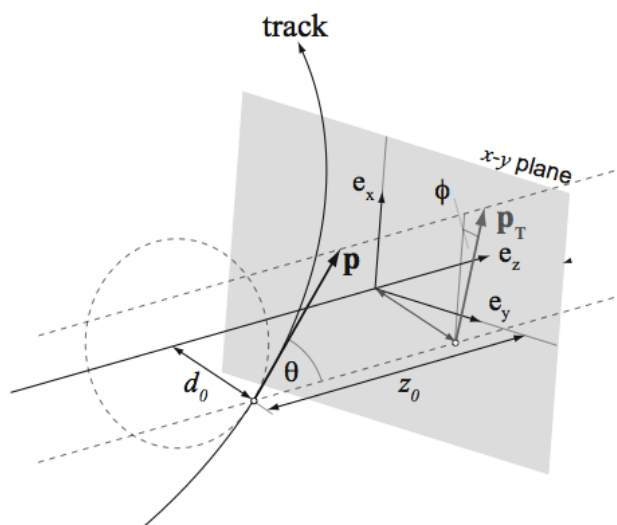
\includegraphics[width=0.6\textwidth]{figures/chapter3/perigee_params}
        \caption{
            Illustration of the relationship between the track parameters and associated track.
            In this scenario, the hard scatter primary vertex is located
            at $(e_x, e_y, e_z) = (0,0,0)$, though this is not generally the case.
        }
        \label{fig:track_params}
    \end{center}
\end{figure}

\begin{figure}[!htb]
    \begin{center}
        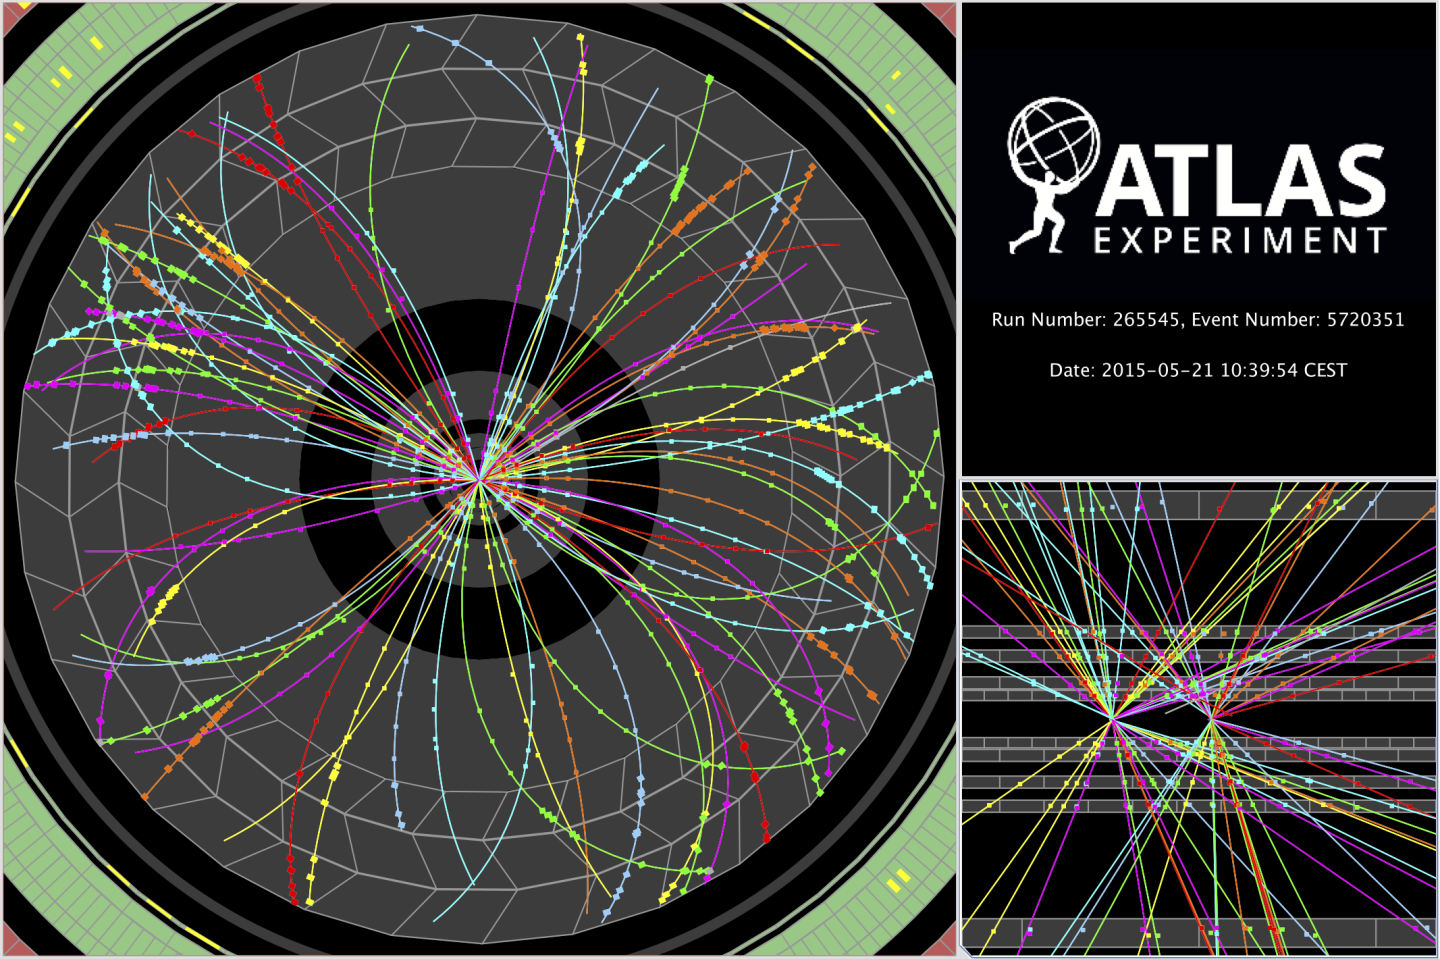
\includegraphics[width=0.7\textwidth]{figures/chapter3/event_display_tracking_vertexing}
        \caption{
            Event display of a low-pileup event recorded at the start of Run 2, in early 2015.
            \textbf{\textit{Left}}: Transverse view of the ID. Seen in color are the reconstructed tracks traversing
                the inner layers of the pixel detector, SCT, and TRT. The colored dots are all reconstructed
                spacepoints used as input to the track fitting procedure.
            \textbf{\textit{Right,\,lower}}: View in $r-z$ of the same $pp$ bunch-crossing event as on the left.
                Two reconstructed primary vertices are clearly observed.
                On average, in Run 2 there were roughly 30 primary vertices reconstructed per event, with
                up to $\approx65$ occurring at maximum.
        }
        \label{fig:id_event_display}
    \end{center}
\end{figure}
\FloatBarrier
